\chapter{Hash-Funktionen}

Die Anforderungen an eine kryptographische Hashfunktion sind:
\begin{itemize}
    \item Kompression, d.h. ein beliebig langer Input wird auf einen Output fixer Länge gemappt
    \item Einwegfunktion (preimage resistance), d.h. gegeben $y = h(x)$ ist es schwierig, das verwendete $x$ zu bestimmen
    \item Schwache Kollisionsresistenz (2nd preimage resistance), d.h. gegeben $x$ mit $y = h(x)$ ist es schwierig, ein $x' \neq x$ zu finden, so dass $h(x) = h(x')$
    \item Starke Kollisionsresistenz (collision resistance), d.h. es ist schwierig, zwei $x$ und $x'$ zu finden, mit $x \neq x'$, so dass $h(x) = h(x')$
\end{itemize}

\section{Konstruktion}

Grundsätzlich sind für eine Hashfunktion zwei Komponenten nötig, eine Kompressionsfunktion, die längere Inputs auf die gewünschte Länge komprimieren, und ein Domain 
Extender, der aus Funktionen mit Eingaben fester Länge Funktionen mit Eingabe beliebiger Länge macht.

\paragraph{Kompressionsfunktionen} haben für einen fixen Input $m$ einen fixen Output $n$ mit $|m| > |n|$.

Es wird entweder eine eigens für den Hash geschriebene Funktion verwendet, z.B. bei MD5 und SHA-1, SHA-2, SHA-3, oder es wird ein Blockcipher eingesetzt. Bei einem 
Blockcipher wird ein Input der Länge $k+l$ (Länge des Schlüssels und Länge des Klartexts) auf einen Input der Länge $l$ gemappt. \\

Die zwei häufigsten Konstruktionen sind
\begin{itemize}
    \item Davis-Meyer: $h(x, y) = E_y(x) \oplus y$
    \item Miyaguchi-Preneel: $h(x, y) = E_x(y) \oplus x \oplus y$
\end{itemize}



\paragraph{Domain Extender} machen aus einer Funktion, die nur Inputs mit einer fixen Länge $n$ nimmt, eine Funktion die Inputs mit beliebiger Länge nimmt. 

Mehr oder weniger alle modernen Hashfunktionen folgen diesem Prinzip:

\begin{enumerate}
    \item Input wird in Blöcke $x_1, \ldots, x_n$ gleicher Länge aufgespalten
    \item Jeder Block dient als Input einer Einweg-Kompressionsfunktion $f$
    \item Input des $i$-ten Funktionsaufrufs sind das vorherige Ergebnis $h_{i-1}$ und der $i$-te Nachrichtenblock $x_i$
    \begin{itemize}
        \item $h_i = f(h_{i-1}, x_i)$
        \item $h(x) = h_{n+1}$ für eine Nachricht mit {n} Blöcken
        \item $h_i$ ist der interne Zustand der Hashfunktion
    \end{itemize}
    \item Ist die verwendete Funktion $f$ kollisionsresistent, so gilt das auch für $h$
    \item Im letzten Block der zu hashenden Nachricht wird die Länge der Originalnachricht angehängt, damit gleich endende aber unterschiedlich lange Nachrichten 
    unterschiedliche Hashwerte ergeben, z.B. \verb|Foo0| vs. \verb|Foo00|
    \item Grundproblem der Konstruktion: Length Extension Attack
    \begin{itemize}
        \item Kompletter interner State ist in Hashwert enthalten
        \item Falls MAC Konstruktion der Form H(key||Nachricht) ist, kann leicht Hashwert für verlängerte Nachricht konstruiert werden
    \end{itemize}
\end{enumerate}

\section{Algebraische Hashfunktionen}

In der Praxis werden aus Geschwindigkeitsgründen hauptsächlich Hashfunktionen
basierend auf logischen Funktionen verwendet. Algebraische Funktionen sind kaum verbreitet, sie basieren auf ähnlichen Argumentationen wie
Public-Key Kryptographie (vgl. AES vs. RSA), also z.B. dem DLP (Discrete Logarithm Problem). Für die Hashfunktion gilt 

$$h(x) = g^x \mod p,$$

wobei das Umkehren der Funktion äquivalent zum Lösen des diskreten Logarithmusproblems ist.
Es gibt auch Hashfunktionen basierend auf RSA

$$H(x) = g^x \mod n (\text{mit } n = p\cdot q),$$

wo das Umkehren der Funktion äquivalent zum Lösen des RSA Problems ist.

\section{MD5} wurde 1991 von Ron Rivest als verbesserter Nachfolger zu MD4 erfunden.

\begin{itemize}
    \item 1996 erste Fehler entdeckt, 2004 weitere Schwachstellen gefunden
    \item 2007 Methoden vorgestellt, um 2 Dateien mit selber MD5 Checksumme zu erzeugen
    \item 2008 gefälschte SSL Zertifikate mit dieser Methode erzeugt
    \item 2008: ``Software developers, Certification Authorities, website owners, and users should avoid using the MD5 algorithm in any capacity. As previous research 
    has demonstrated, it should be considered cryptographically broken and unsuitable for further use.'' -- US-CERT, \url{http://www.kb.cert.org/vuls/id/836068}
\end{itemize}

Die Funktion erzeut in 64 Operationen (in 4 Runden zu je 16 Operationen) einen Output der Länge 128.

\begin{enumerate}
    \item Nachricht wird in 512 Bit große Blöcke aufgespalten und gepadded (siehe Kapitel ``Padding'')
    \item der interne State hat 128 Bit, wird in 4 32-Bit Wörtern gehalten. Er wird mit \verb|01 23 45 67|, \verb|89 ab cd ef|, \verb|fe dc ba 98|, \verb|76 54 32 10|, 
    sogenannte ``nothing up my sleeve'' numbers
    \item es gibt eine additive Rundenkonstante: in Runde $i$ wird $K_i = 2^{32}\cdot|\sin(i)|$ addiert 
    \item Alle 16 Operationen wechselt die Rundenfunktion ($F$, $G$, $H$, $I$)
    \begin{itemize}
        \item F(X,Y,Z) = (X and Y) or (not X and Z)
        \item G(X,Y,Z) = (X and Z) or (Y and not Z)
        \item H(X,Y,Z) = X $\oplus$ Y $\oplus$ Z
        \item I(X,Y,Z) = Y $\oplus$ (X or not Z)
    \end{itemize}
    \item Jede Runde um anderen Offset zirkulär geshiftet
\end{enumerate}

\begin{figure}[h]
    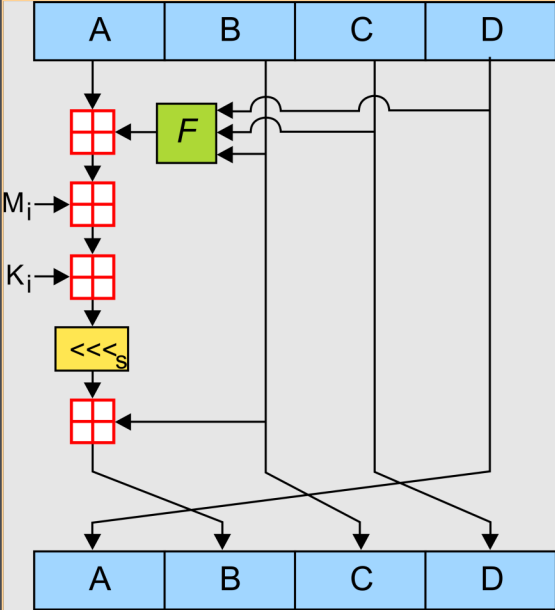
\includegraphics[width=0.4\textwidth]{figures/fig09-md5}
    \centering
    \caption{MD5 Operation, die 64 Mal wiederholt wird}
\end{figure}


\section{SHA (Secure Hash Algorithm)}

1993 wurde SHA-0 veröffentlicht, 1995 dann der verbesserte SHA-1 und 2001 SHA-2. Das NIST hat SHA-3 ausgeschrieben, das Ende des Auswahlprozesses war 2012 (vgl. AES).
Dann wurde Keccak als SHA-3 2015 standardisiert. \\

\paragraph{SHA-1}
Der SHA-1 mit voller Rundenzahl gilt seit 2005 als unsicher. Kollisionen können mit $2^{63}$ Operationen erzeugt werden, 2008 wurde die Zahl auf $2^{51}$ verringert.
Seit 2017 sind Kollisionen in 2 validen PDF Dokumenten konstruierbar. \\

Er erzeugt einen 160 Bit Output und basiert auf denselben Grundideen wie MD4 und MD5:

\begin{itemize}
    \item Nachricht ebenfalls in 512-Bit Blöcke gespalten
    \item es gibt 80 Runden, alle 20 Runden wechselt die Rundenfunktion
    \begin{enumerate}
        \item F(X,Y,Z) = (X and Y) or (not X and Z) (ident zu MD5)
        \item G(X,Y,Z) = X $\oplus$ Y $\oplus$ Z (ident zu H aus MD5)
        \item H(X,Y,Z) = (X and Y) or (X and Z) or (Y and Z)
        \item I(X,Y,Z) = G (sic)
    \end{enumerate}
    \item es gibt 4 Rundenkonstanten
    \begin{enumerate}
        \item $K_1 = 230 \cdot \sqrt(2)$ 
        \item $K_2 = 230 \cdot \sqrt(3)$
        \item $K_3 = 230 \cdot \sqrt(5)$
        \item $K_4 = 230 \cdot \sqrt(10)$
    \end{enumerate}
    \item In jeder Runde um 30 zirkulär geshiftet
\end{itemize}

\paragraph{SHA-2} beschreibt eine Familie an Hashfunktionen, die die Algorithmen SHA-224, SHA-256, SHA-384, SHA-512, SHA-512/224 und SHA-512/256. Sie sind im FIPS 
(Federal Information Processing Standards) PUB-180-4 beschrieben.


\begin{center}
    \begin{tabular}{ llll } 
        \hline
        Algorithmus & Ausgabegröße (Bit) & Interne Blockgröße (Bit) & basiert auf \\ 
        \hline
        SHA-224     & 224 &  512 & SHA-256\\
        SHA-256     & 256 &  512 & SHA-256\\
        SHA-384     & 384 & 1024 & SHA-512\\
        SHA-512     & 512 & 1024 & SHA-512\\
        SHA-512/224 & 224 & 1024 & SHA-512\\
        SHA-512/256 & 256 & 1024 & SHA-512\\
        \hline
    \end{tabular}
\end{center}

\subparagraph{SHA-224}: Kürzere Version von SHA-256 mit 224 Bit Ausgabelänge. Geeignet, wenn Speicher knapp ist, z.B. constraint devices (Memory).
\subparagraph{SHA-256}: Der meistverwendete SHA-2-Algorithmus. Standard für viele Anwendungen (z. B. TLS, digitale Signaturen)
\subparagraph{SHA-384}: Abgespeckte Version von SHA-512 mit anderer Initialisierung und kürzerer Ausgabe.
\subparagraph{SHA-512}: Sicherste (längste) Standardvariante mit 512 Bit Ausgabelänge.
\subparagraph{SHA-512/224} (constraint devices (Memory)), siehe SHA-512/256.  
\subparagraph{SHA-512/256} (allg. Sicherheit): Truncate-Versionen von SHA-512 mit kürzerer Ausgabelänge. Bietet eine Kombination aus höherer
Sicherheit (wegen 1024-Bit Blockgröße) und kürzeren Hashes.

\section{Merkle-Damgard}
\section{SHA-3}
\section{Angriffe}


% \begin{itemize}
% \end{itemize}

% \begin{enumerate}
% \end{enumerate}

% \begin{align*}
% \end{align*}
